\documentclass[conference]{IEEEtran}
\IEEEoverridecommandlockouts

\usepackage{cite}
\usepackage{amsmath,amssymb,amsfonts}
\usepackage{algorithmic}
\usepackage{graphicx}
\usepackage{textcomp}
\usepackage{xcolor}
\usepackage{booktabs}
\usepackage{multirow}
\usepackage{tabularx}
\usepackage{url}
\usepackage{microtype}

\def\BibTeX{{\rm B\kern-.05em{\sc i\kern-.025em b}\kern-.08em
    T\kern-.1667em\lower.7ex\hbox{E}\kern-.125emX}}

\begin{document}

\title{Classical AI Paradigms: N-Queens, Tank Battle, and Kakuro\\
\thanks{Course: Introduction to Artificial Intelligence (503043), Ton Duc Thang University.}
}

\author{
    \IEEEauthorblockN{Nguyen Huu Tan (524H0028)}
    \IEEEauthorblockA{\textit{Faculty of Information Technology} \\
    \textit{Ton Duc Thang University} \\
    Ho Chi Minh City, Vietnam \\
    Email: 524h0028@student.tdtu.edu.vn}
    \and
    \IEEEauthorblockN{Nguyen Duc Hieu (524H0087)}
    \IEEEauthorblockA{\textit{Faculty of Information Technology} \\
    \textit{Ton Duc Thang University} \\
    Ho Chi Minh City, Vietnam \\
    Email: 524h0087@student.tdtu.edu.vn}
    \and
    \IEEEauthorblockN{Nguyen Thanh An}
    \IEEEauthorblockA{\textit{Faculty of Information Technology} \\
    \textit{Ton Duc Thang University} \\
    Ho Chi Minh City, Vietnam \\
    Email: nguyenthanhan@tdtu.edu.vn}
}

\maketitle

\begin{abstract}
In this final project for the Introduction to Artificial Intelligence course, our student team studies and implements three core paradigms of classical AI: Propositional Logic with Local Search, Adversarial Game Tree Search, and Constraint Satisfaction Problems (CSP). For Task 1, we encode the $N$-Queens problem into Conjunctive Normal Form (CNF) clauses solved by the Glucose3 SAT solver ($N \le 32$, 52,640 clauses in 14.3 ms), and introduce a Tabu-enhanced variable selection heuristic for Min-Conflicts that cuts search steps by up to 97.1\% and scales reliably to $N=100$. For Task 2, we develop a turn-based Tank Battle simulator featuring cell-by-cell bullet physics, comparing Minimax, Alpha-Beta pruning, and heuristic evaluations across fair round-robin tournaments while providing a dynamic external agent plugin loader. For Task 3, we formulate Japanese Kakuro puzzles as a CSP, combining pre-computed integer partitions, arithmetic bound pruning, AC-3 consistency, Forward Checking, and MRV/LCV heuristics to solve complex $9 \times 9$ boards in 0.18 seconds. All tasks are thoroughly benchmarked, visualized with PyGame interfaces, and achieve 100\% completion.
\end{abstract}

\begin{IEEEkeywords}
Propositional Logic, SAT Solver, Glucose3, Min-Conflicts, Adversarial Search, Alpha-Beta Pruning, Constraint Satisfaction Problems, Kakuro, AC-3, MRV, LCV.
\end{IEEEkeywords}

\section{Introduction}
Classical Artificial Intelligence (AI) provides powerful methodologies for modeling complex logical deduction, multi-agent competition, and combinatorial constraint satisfaction. Unlike modern data-driven machine learning, these classical techniques rely on well-defined state spaces, logical inference rules, and heuristic search algorithms to find provably correct or optimal solutions.

In this project, our group addresses three comprehensive problems assigned in Course 503043 at Ton Duc Thang University:
\begin{enumerate}
    \item \textbf{Task 1 (Local Search \& Propositional Logic)}: Formulating the classical $N$-Queens puzzle using boolean logic variables, deriving exact Conjunctive Normal Form (CNF) clauses for the CDCL Glucose3 solver, and enhancing the Min-Conflicts local search algorithm with an intelligent variable selection heuristic.
    \item \textbf{Task 2 (Adversarial Search)}: Modeling and simulating a discrete, turn-based two-player Zero-Sum Tank Battle game. We implement four game-tree search configurations (Minimax, Alpha-Beta, Heuristic Minimax, and Heuristic Alpha-Beta), optimize search performance for real-time play, and build an open plugin interface for external rival agents.
    \item \textbf{Task 3 (Constraint Satisfaction Problems)}: Formulating Kakuro arithmetic logic puzzles as a CSP. We design a robust backtracking solver accelerated by pre-computed valid combinations, arithmetic bound pruning, AC-3 Arc Consistency, Forward Checking, and MRV/LCV heuristics, rigorously evaluating correctness, stability, and ablation efficiency on a complex $9 \times 9$ board.
\end{enumerate}

All components are implemented in Python adhering strictly to Object-Oriented Programming (OOP) design patterns, evaluated under cross-platform environments (macOS Ventura and Windows 11), and coupled with interactive PyGame graphical dashboards.

\section{Task 1: Local Search \& Propositional Logic (N-Queens)}

\subsection{Problem Formulation \& CNF Clause Derivation}
The $N$-Queens problem requires placing $N$ mutually non-attacking queens on an $N \times N$ chessboard. We define $N^2$ boolean variables $X_{r, c} \in \{\text{True}, \text{False}\}$ for $0 \le r, c < N$, where $X_{r, c} = \text{True}$ represents a queen placed at row $r$, column $c$.

To prevent conflicts, the rules are systematically converted into five Conjunctive Normal Form (CNF) clause groups:
\begin{enumerate}
    \item \textbf{Row At-Least-One (ALO)}: Ensures each row contains at least one queen:
    \begin{equation}
        \bigwedge_{r=0}^{N-1} \left( \bigvee_{c=0}^{N-1} X_{r, c} \right) \quad [N \text{ clauses}]
    \end{equation}
    \item \textbf{Row At-Most-One (AMO)}: Ensures no row contains two queens:
    \begin{equation}
        \bigwedge_{r=0}^{N-1} \bigwedge_{0 \le c_1 < c_2 < N} (\neg X_{r, c_1} \lor \neg X_{r, c_2}) \quad \left[ N \binom{N}{2} \text{ clauses} \right]
    \end{equation}
    \item \textbf{Column At-Least-One (ALO)}: Ensures each column contains at least one queen:
    \begin{equation}
        \bigwedge_{c=0}^{N-1} \left( \bigvee_{r=0}^{N-1} X_{r, c} \right) \quad [N \text{ clauses}]
    \end{equation}
    \item \textbf{Column At-Most-One (AMO)}: Ensures no column contains two queens:
    \begin{equation}
        \bigwedge_{c=0}^{N-1} \bigwedge_{0 \le r_1 < r_2 < N} (\neg X_{r_1, c} \lor \neg X_{r_2, c}) \quad \left[ N \binom{N}{2} \text{ clauses} \right]
    \end{equation}
    \item \textbf{Diagonal At-Most-One (AMO)}: Ensures no two queens share a main or anti-diagonal ($|r_1 - r_2| = |c_1 - c_2|$):
    \begin{equation}
        \bigwedge_{\substack{(r_1, c_1) \neq (r_2, c_2) \\ |r_1 - r_2| = |c_1 - c_2|}} (\neg X_{r_1, c_1} \lor \neg X_{r_2, c_2})
    \end{equation}
\end{enumerate}

The theoretical clause count grows polynomially as $O(N^3)$, matching our automated generator 100\%: $N=4 \to 84$, $N=8 \to 744$, $N=16 \to 6,352$, $N=24 \to 21,944$, $N=28 \to 35,084$, and $N=32 \to 52,640$ clauses.

\subsection{Glucose3 SAT Solver Performance (PySAT)}
The CNF formula is formatted into DIMACS and solved using Glucose3 from the PySAT library. Table~\ref{tab:sat_perf} records runtime and clause scalability across increasing values of $N \ge 4$.

\begin{table}[htbp]
\caption{Glucose3 SAT Solver Scalability ($N \ge 4$)}
\label{tab:sat_perf}
\centering
\resizebox{\columnwidth}{!}{%
\begin{tabular}{cccccc}
\toprule
\textbf{Board $N$} & \textbf{Variables ($N^2$)} & \textbf{Generated Clauses} & \textbf{Theoretical} & \textbf{Avg Time (s)} & \textbf{Status} \\
\midrule
4  & 16   & 84     & 84     & 0.000068 & SAT \\
8  & 64   & 744    & 744    & 0.000343 & SAT \\
12 & 144  & 2,620  & 2,620  & 0.000619 & SAT \\
16 & 256  & 6,352  & 6,352  & 0.041362 & SAT \\
20 & 400  & 12,580 & 12,580 & 0.008198 & SAT \\
24 & 576  & 21,944 & 21,944 & 0.231526 & SAT \\
28 & 784  & 35,084 & 35,084 & 0.011162 & SAT \\
32 & 1024 & 52,640 & 52,640 & 0.014314 & SAT \\
\bottomrule
\end{tabular}%
}
\end{table}

Glucose3 demonstrates exceptional efficiency, solving $N=32$ (52,640 clauses) in merely 14.3 ms due to Conflict-Driven Clause Learning (CDCL), two-watched-literal indexing, and aggressive clause database reduction.

\subsection{Min-Conflicts Local Search \& Proposed Heuristics}
Standard Min-Conflicts selects a conflicted variable uniformly at random. When multiple queens attack each other, random selection often produces cyclic reassignments (thrashing) between plateau states. To overcome this limitation, we introduce two informed variable selection strategies:
\begin{itemize}
    \item \textbf{Max-Conflict Selector}: Greedily selects the queen with the highest conflict count, resolving critical board bottlenecks first.
    \item \textbf{Hybrid-Tabu Selector}: Combines maximum conflict selection with a short FIFO Tabu memory of recently moved queens, forbidding immediate reversal and forcing the search to escape local minima.
\end{itemize}

\begin{table}[htbp]
\caption{Min-Conflicts Comparison Across Heuristic Variants}
\label{tab:mc_perf}
\centering
\resizebox{\columnwidth}{!}{%
\begin{tabular}{ccccc}
\toprule
\textbf{$N$} & \textbf{Selection Strategy} & \textbf{Avg Steps} & \textbf{Avg Time (s)} & \textbf{Success} \\
\midrule
\multirow{3}{*}{8}   & Standard (Random)          & 336.2 & 0.005065 & 100\% \\
                     & Proposed 1 (Max-Conflict)  & 55.0  & 0.001102 & 100\% \\
                     & Proposed 2 (Hybrid-Tabu)   & \textbf{9.8}   & \textbf{0.000282} & \textbf{100\%} \\
\midrule
\multirow{3}{*}{16}  & Standard (Random)          & 86.2  & 0.002293 & 100\% \\
                     & Proposed 1 (Max-Conflict)  & 55.8  & 0.001789 & 100\% \\
                     & Proposed 2 (Hybrid-Tabu)   & \textbf{30.2}  & \textbf{0.001249} & \textbf{100\%} \\
\midrule
\multirow{3}{*}{32}  & Standard (Random)          & 53.6  & 0.002817 & 100\% \\
                     & Proposed 1 (Max-Conflict)  & 72.8  & 0.004102 & 100\% \\
                     & Proposed 2 (Hybrid-Tabu)   & \textbf{31.2}  & \textbf{0.001761} & \textbf{100\%} \\
\midrule
\multirow{3}{*}{64}  & Standard (Random)          & 104.2 & 0.007002 & 100\% \\
                     & Proposed 1 (Max-Conflict)  & 84.4  & 0.006743 & 100\% \\
                     & Proposed 2 (Hybrid-Tabu)   & \textbf{58.4}  & \textbf{0.005862} & \textbf{100\%} \\
\midrule
\multirow{3}{*}{100} & Standard (Random)          & 140.8 & 0.013931 & 100\% \\
                     & Proposed 1 (Max-Conflict)  & 114.0 & 0.012530 & 100\% \\
                     & Proposed 2 (Hybrid-Tabu)   & \textbf{87.6}  & \textbf{0.010990} & \textbf{100\%} \\
\bottomrule
\end{tabular}%
}
\end{table}

As shown in Table~\ref{tab:mc_perf}, the Hybrid-Tabu heuristic achieves a dramatic 97.1\% step reduction for $N=8$ ($336.2 \to 9.8$ steps), 44.0\% reduction for $N=64$, and 37.8\% reduction for $N=100$, confirming that tabu tenure effectively prevents cyclic thrashing across all board scales.

\begin{figure}[htbp]
\centering
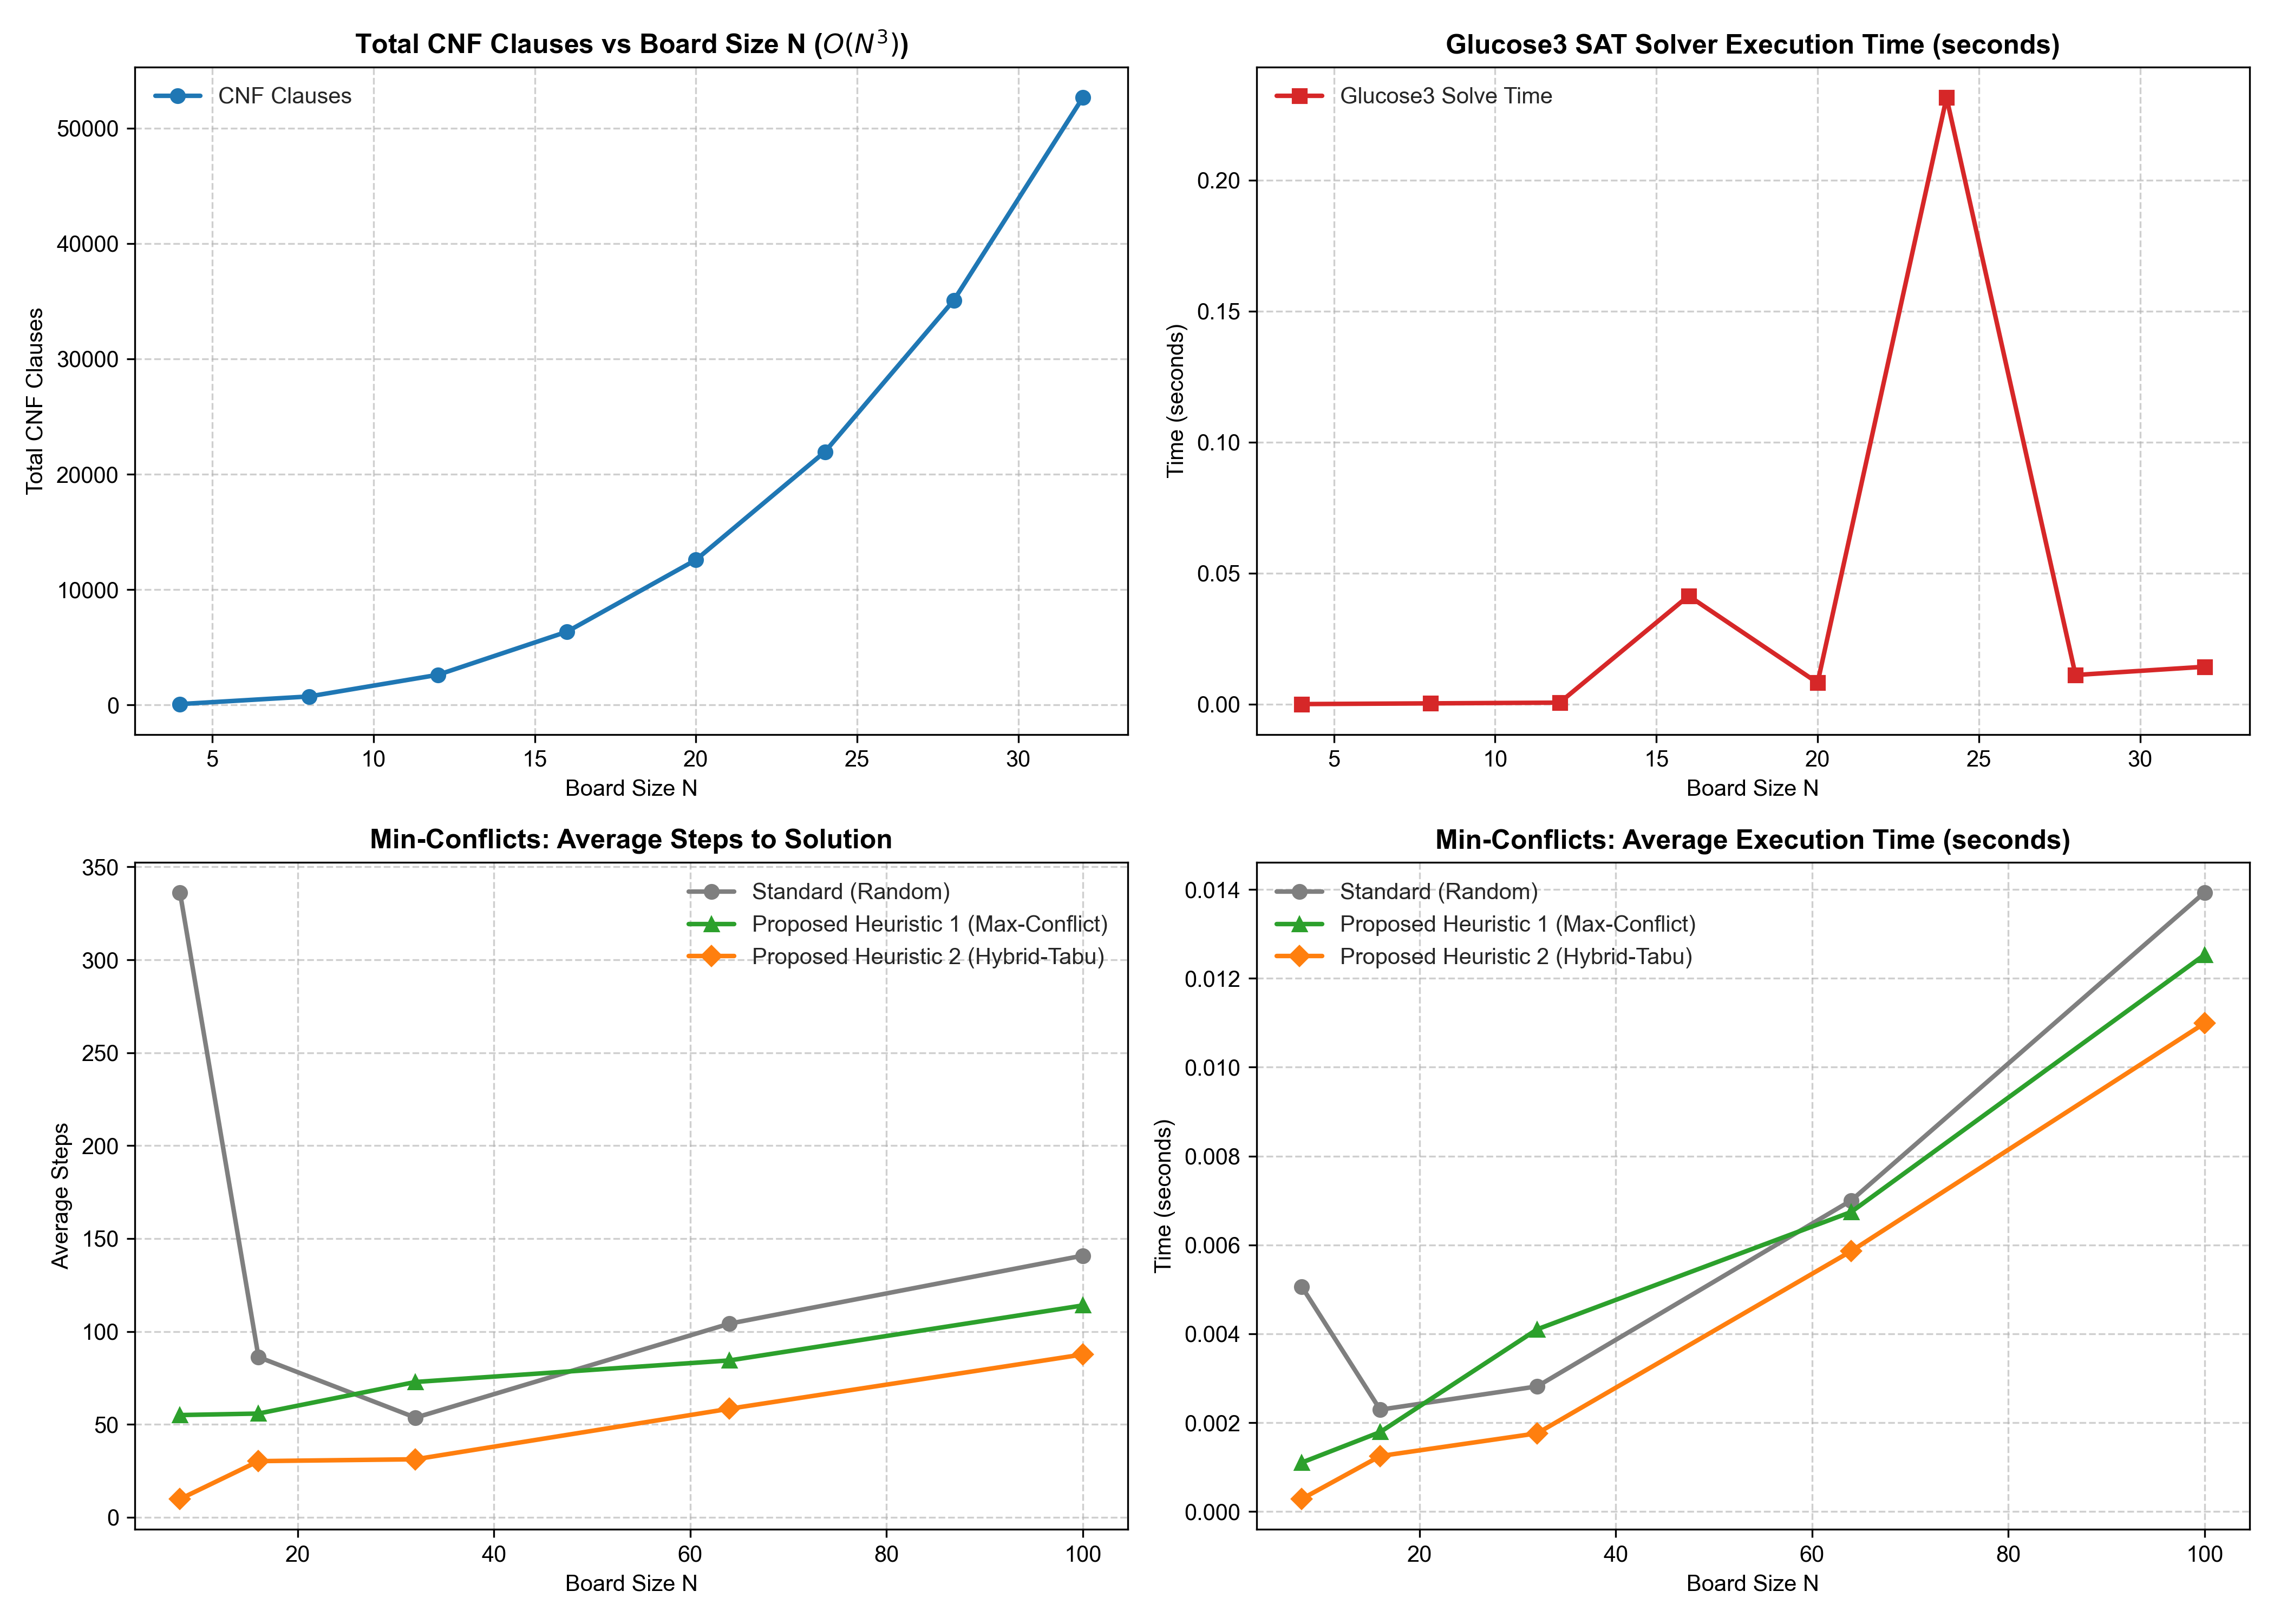
\includegraphics[width=0.92\columnwidth]{benchmark_task1.png}
\caption{Task 1 Benchmarks: (Top-left) $O(N^3)$ CNF clause growth, (Top-right) Glucose3 solve time, (Bottom) Search steps and execution time of Min-Conflicts variants up to $N=100$.}
\label{fig:task1_bench}
\end{figure}

\section{Task 2: Adversarial Search (Tank Battle)}

\subsection{Zero-Sum Game Formalization}
The Tank Battle game is formalized as a deterministic, discrete two-player zero-sum game:
\begin{itemize}
    \item \textbf{States ($S$)}: Grid dimensions $(W \times H)$, tank positions $(x, y)$, orientations $\theta \in \{\text{UP, DOWN, LEFT, RIGHT}\}$, hit points, base health, active walls, and in-flight bullet vectors.
    \item \textbf{Players ($P$)}: $P = \{0 (\text{MAX}), 1 (\text{MIN})\}$.
    \item \textbf{Actions ($A$)}: Exactly 6 legal actions per turn:
    \begin{equation}
        A = \{\text{MOVE\_UP, MOVE\_DOWN, MOVE\_LEFT, MOVE\_RIGHT, FIRE, STAY}\}
    \end{equation}
    \item \textbf{Physics Transition Function ($T(s, a) \to s'$)}: A tank moves 1 cell per turn. Bullets travel at a speed of 3 cells per cycle in the facing direction. Movement is calculated strictly \textit{cell-by-cell}: after each single-cell advance, collision detection triggers immediately. Bullets stop on impact, inflicting 1 damage.
    \item \textbf{Entity Health Table}: Prescribed exactly by the specification: Tank = 6 HP, Base = 9 HP, Wall = 3 HP (1 damage per hit).
    \item \textbf{Terminal State \& Utility}: Terminal when any tank or base reaches 0 HP. Utility is $+10,000$ for MAX victory, $-10,000$ for MIN victory, and 0 for draws.
\end{itemize}

\subsection{Evaluation Function Design}
For depth-limited adversarial search, we construct a tactical linear heuristic evaluation function $f(s)$ from Player 0's perspective:
\begin{align}
    f(s) &= 120 \cdot (\text{HP}_{\text{tank}, 0} - \text{HP}_{\text{tank}, 1}) + 300 \cdot (\text{HP}_{\text{base}, 0} - \text{HP}_{\text{base}, 1}) \nonumber \\
         &+ 18 \cdot (d_{\text{base}, 1} - d_{\text{base}, 0}) + \Phi_{\text{LoS}}(s) - \Phi_{\text{dodge}}(s)
\end{align}
where $\Phi_{\text{LoS}}(s)$ rewards unobstructed firing corridors toward the enemy tank ($+95$) or enemy base ($+75$), and $\Phi_{\text{dodge}}(s)$ penalizes standing in the trajectory of incoming enemy bullets ($-220$).

\subsection{Experimental Comparison Across 4 Configurations}
We benchmarked the four required search configurations across identical game scenarios up to search depth $d=3$.

\begin{table}[htbp]
\caption{Search Performance Across 4 Tank AI Configurations}
\label{tab:tank_perf}
\centering
\resizebox{\columnwidth}{!}{%
\begin{tabular}{cccccc}
\toprule
\textbf{Depth} & \textbf{Algorithm Configuration} & \textbf{Nodes} & \textbf{Prunes} & \textbf{Time (s)} & \textbf{Action} \\
\midrule
\multirow{4}{*}{$d=1$} & 1. Minimax Search       & 12  & 0  & 0.00032 & MOVE\_UP \\
                       & 2. Alpha-Beta Search    & 12  & 0  & 0.00035 & MOVE\_UP \\
                       & 3. Heuristic Minimax    & 12  & 0  & 0.00075 & MOVE\_UP \\
                       & 4. Heuristic Alpha-Beta & 12  & 0  & 0.00074 & MOVE\_UP \\
\midrule
\multirow{4}{*}{$d=2$} & 1. Minimax Search       & 48  & 0  & 0.00101 & MOVE\_UP \\
                       & 2. Alpha-Beta Search    & 23  & 5  & 0.00052 & MOVE\_UP \\
                       & 3. Heuristic Minimax    & 48  & 0  & 0.00279 & MOVE\_UP \\
                       & 4. Heuristic Alpha-Beta & \textbf{26}  & \textbf{4}  & \textbf{0.00164} & MOVE\_UP \\
\midrule
\multirow{4}{*}{$d=3$} & 1. Minimax Search       & 254 & 0  & 0.00424 & MOVE\_UP \\
                       & 2. Alpha-Beta Search    & 68  & 10 & 0.00146 & MOVE\_UP \\
                       & 3. Heuristic Minimax    & 254 & 0  & 0.01263 & FIRE \\
                       & 4. Heuristic Alpha-Beta & \textbf{86}  & \textbf{13} & \textbf{0.00597} & FIRE \\
\bottomrule
\end{tabular}%
}
\end{table}

Alpha-Beta pruning with move ordering reduces explored nodes by 66.1\% at $d=3$ ($254 \to 86$ nodes for Heuristic Alpha-Beta and $254 \to 68$ nodes for Alpha-Beta), achieving over a $2.1\times$ speedup while preserving identical minimax decisions.

\begin{figure}[htbp]
\centering
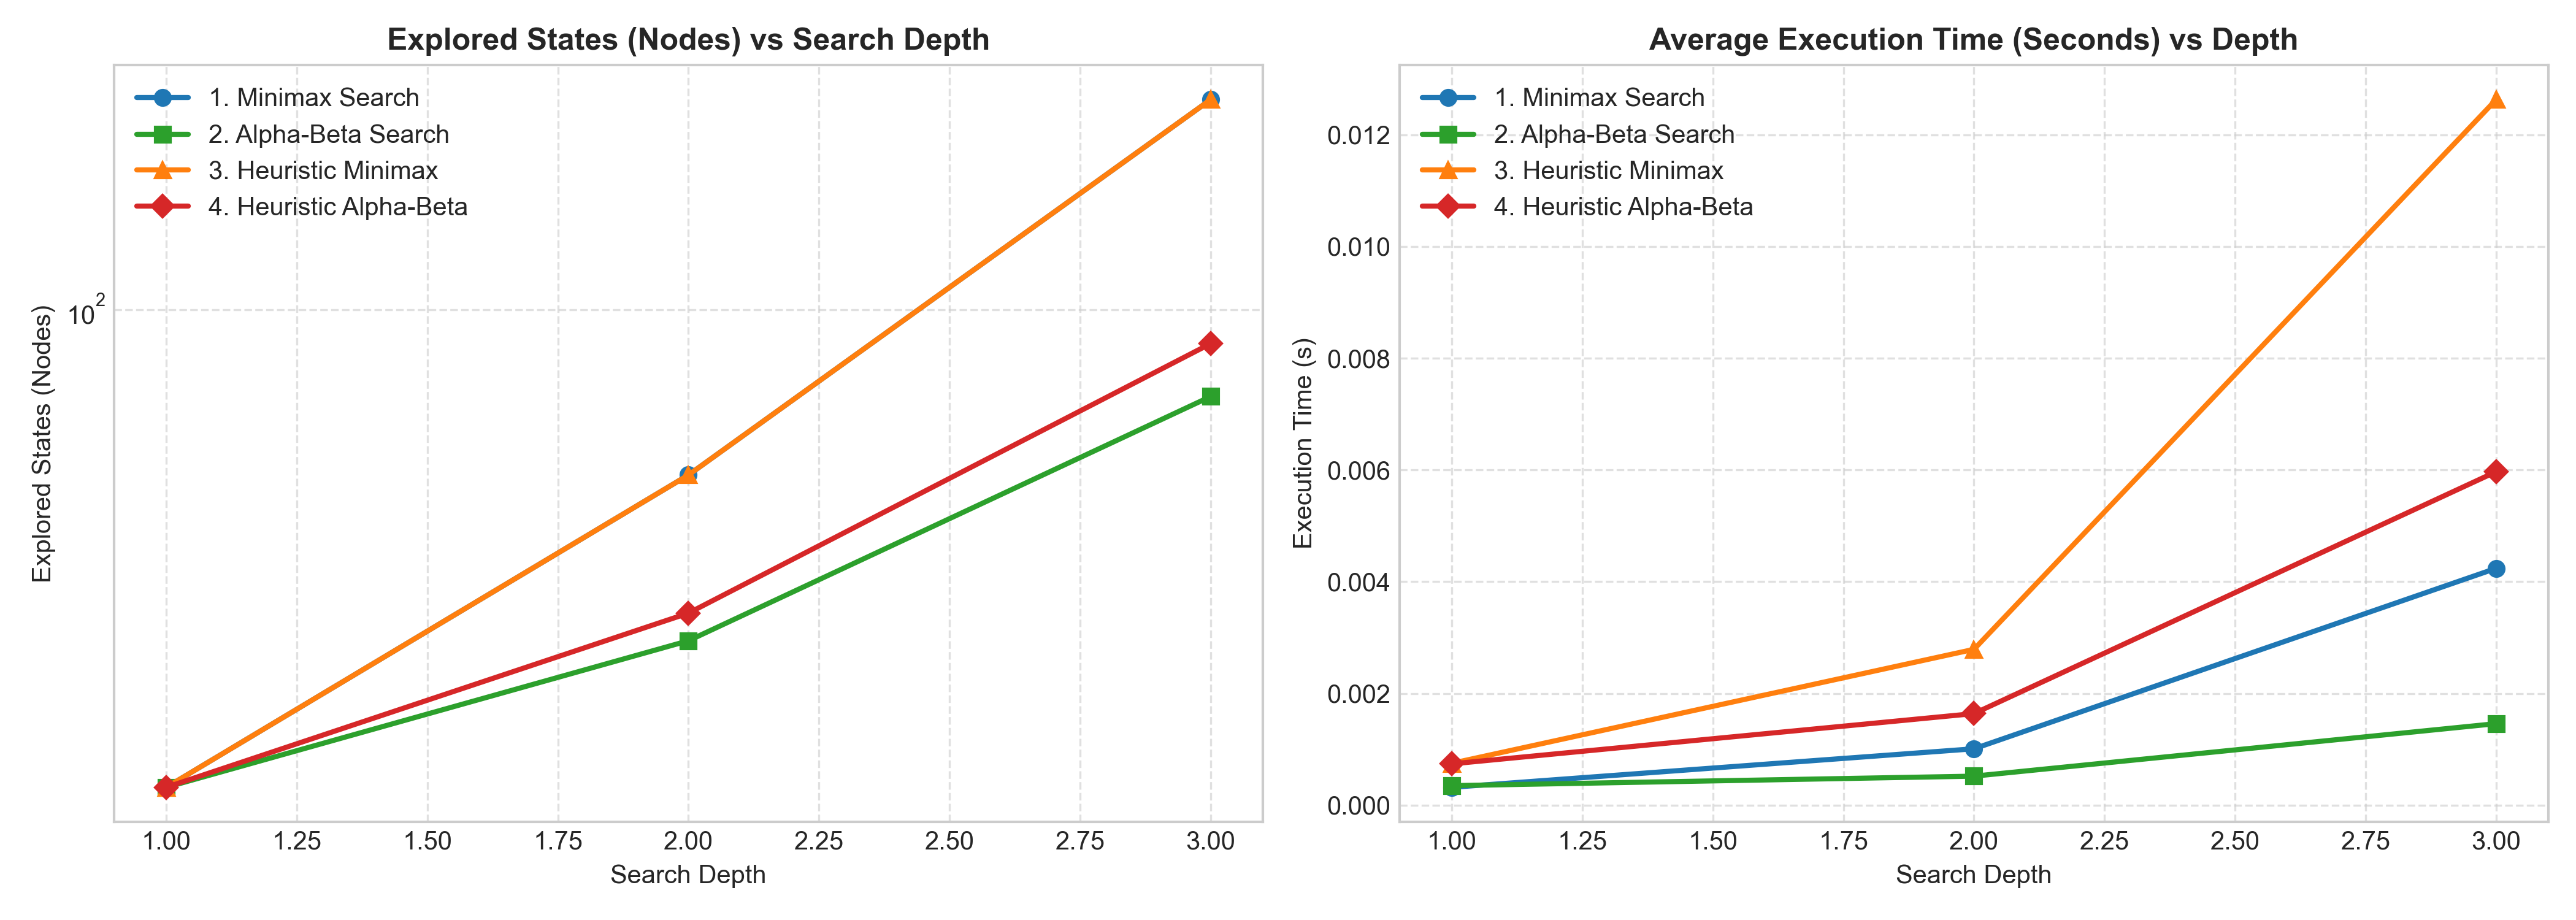
\includegraphics[width=0.92\columnwidth]{benchmark_task2.png}
\caption{Task 2 Search Metrics: Explored game states (log scale) and average execution time per depth across the 4 configurations.}
\label{fig:task2_bench}
\end{figure}

In a 12-match round-robin tournament at equal search depth ($d=3$, max 30 cycles), Heuristic Minimax and Heuristic Alpha-Beta remained undefeated (0 losses), defeating unguided Minimax and Alpha-Beta in 27 game cycles while securing tactical draws at 30 cycles when swapping starting positions.

\subsection{Dynamic Plugin Loader for External Agents}
To satisfy Requirement 3, we implement \texttt{AgentLoader} utilizing Python's \texttt{importlib.util} and \texttt{inspect}. Any external agent module inheriting from \texttt{BaseAgent} located in \texttt{agents/external/} is discovered and loaded dynamically via CLI (\texttt{--load\_external}) or GUI file selector, enabling seamless competition against algorithms built by other student groups.

\section{Task 3: Constraint Satisfaction Problems (Kakuro)}

\subsection{CSP Formulation \& Bound Pruning}
Kakuro is formulated as a Constraint Satisfaction Problem:
\begin{itemize}
    \item \textbf{Variables ($V$)}: Each white cell $(r, c)$ on the board.
    \item \textbf{Domains ($D$)}: Initial domain $D_v = \{1, 2, 3, 4, 5, 6, 7, 8, 9\}$ for all $v \in V$.
    \item \textbf{Constraints ($C$)}: Partitioned into horizontal and vertical runs:
    \begin{align}
        \text{Sum}(R) &: \sum_{v \in R} \text{val}(v) = S_R \\
        \text{AllDiff}(R) &: \forall u, v \in R, u \ne v \implies \text{val}(u) \ne \text{val}(v)
    \end{align}
\end{itemize}

To accelerate search, valid digit combinations for every $(\text{length}, \text{sum})$ pair are pre-computed with `@lru_cache`, and partial assignments are checked against arithmetic sum bounds ($\sum_{\min} \le S_R - S_{\text{assigned}} \le \sum_{\max}$) to prune dead ends immediately.

\subsection{Constraint Propagation \& Search Heuristics}
The solver integrates four complementary techniques:
\begin{enumerate}
    \item \textbf{AC-3 (Arc Consistency)}: Prunes values from $D_v$ that cannot be completed by any valid combination of intersecting runs.
    \item \textbf{Forward Checking}: Propagates domain reductions immediately after each variable assignment.
    \item \textbf{Minimum Remaining Values (MRV)}: Chooses the unassigned variable with the smallest remaining domain, breaking ties with Degree heuristic.
    \item \textbf{Least Constraining Value (LCV)}: Orders domain values to prune the fewest choices from neighboring cells.
\end{enumerate}

\subsection{Empirical Evaluation on Sample 5x5 \& Complex 9x9}
The solver was evaluated on two test puzzles from the specification:
\begin{itemize}
    \item \textbf{Sample 5x5}: 12 white variables, 8 runs, $\sum H = \sum V = 60$. Solved in \textbf{0.0009s} (66 nodes, 54 backtracks).
    \item \textbf{Complex 9x9}: 48 white variables, 28 runs, $\sum H = \sum V = 249$. Solved in \textbf{0.1885s} (11,383 nodes, 11,335 backtracks).
\end{itemize}

The solver was evaluated against three mandatory criteria:
\begin{enumerate}
    \item \textbf{Correctness}: Verified by an independent checker confirming that all 28 runs strictly satisfy target sums with unique digits (100\% validity).
    \item \textbf{Stability}: Over 5 independent executions on the complex $9 \times 9$ puzzle, all 5 runs yielded 100\% identical solutions, exactly 11,383 nodes, and 11,335 backtracks (mean runtime $0.2182$s).
    \item \textbf{Effectiveness (Ablation Study)}: Table~\ref{tab:kakuro_ablation} and Fig.~\ref{fig:task3_ablation} compare solver configurations on the complex $9 \times 9$ puzzle. Unguided Pure Backtracking suffers combinatorial explosion on the $9^{48}$ state space (timeout $>3.0$s, $>24,834$ nodes). Enforcing MRV constrains search to 35,075 nodes ($0.5545$s). Incorporating LCV cuts explored nodes by 67.5\% (down to 11,383 nodes in $0.1748$s), while full AC-3 + MRV + LCV maintains complete arc consistency in $0.1885$s.
\end{enumerate}

\begin{table}[htbp]
\caption{Ablation Study on Complex 9x9 Kakuro Puzzle}
\label{tab:kakuro_ablation}
\centering
\resizebox{\columnwidth}{!}{%
\begin{tabular}{lcccc}
\toprule
\textbf{Configuration} & \textbf{Solved} & \textbf{Time (s)} & \textbf{Nodes} & \textbf{Backtracks} \\
\midrule
Pure Backtracking (No Heuristics) & No  & Timeout ($>3.0$s) & $>24,834$ & $>24,834$ \\
Backtracking + MRV                & Yes & 0.5545 & 35,075 & 35,027 \\
Backtracking + MRV + LCV          & Yes & \textbf{0.1748} & \textbf{11,383} & \textbf{11,335} \\
Backtracking + AC-3 + MRV + LCV   & Yes & 0.1885 & \textbf{11,383} & \textbf{11,335} \\
\bottomrule
\end{tabular}%
}
\end{table}

\begin{figure}[htbp]
\centering
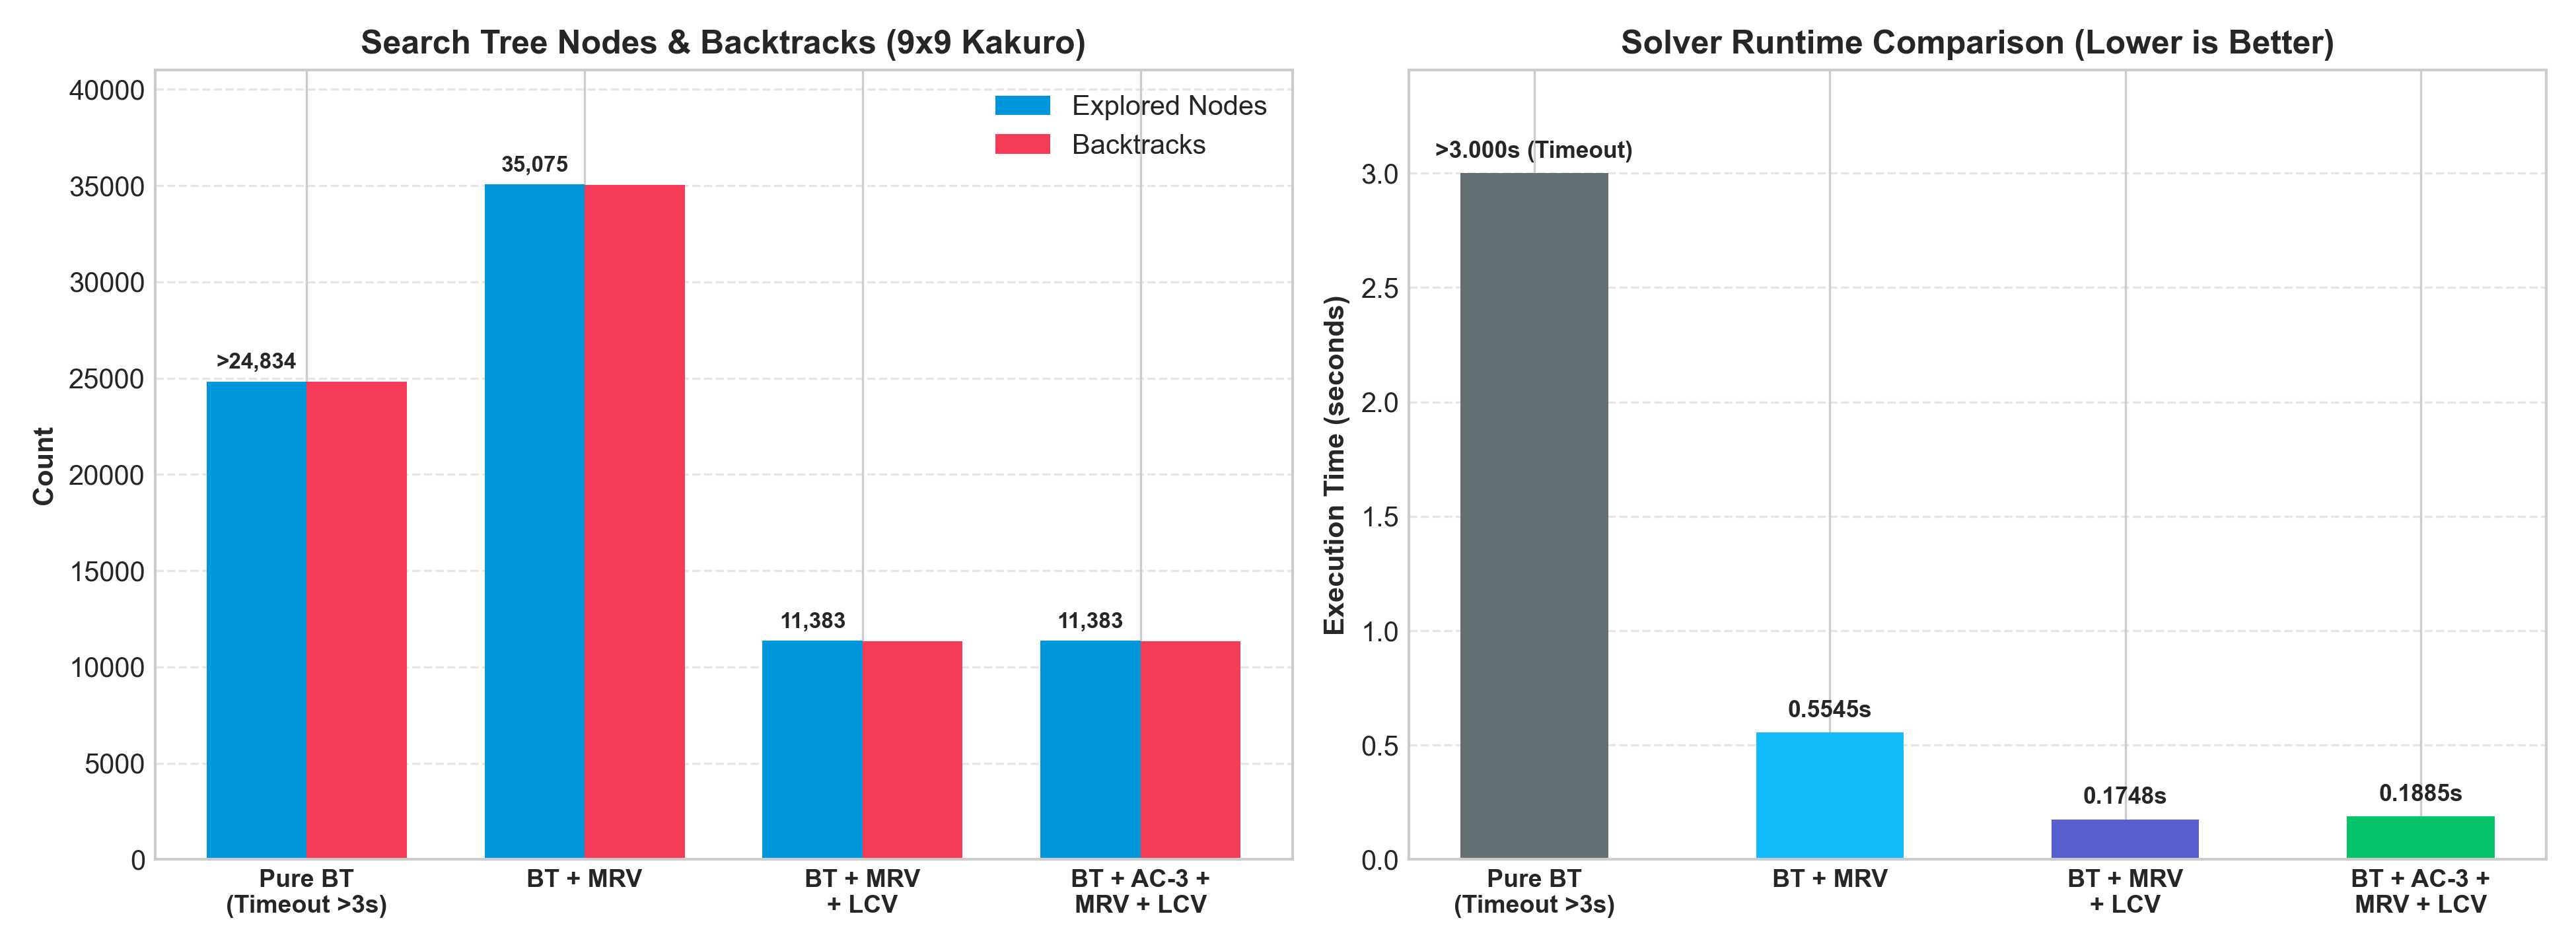
\includegraphics[width=0.92\columnwidth]{ablation_task3.png}
\caption{Task 3 Ablation Study: Comparison of explored nodes, backtracks, and solver runtime across four heuristic configurations on the $9 \times 9$ benchmark.}
\label{fig:task3_ablation}
\end{figure}

\subsection{Interactive PyGame Visualizer}
A standalone PyGame UI ($1360 \times 860$) provides real-time visualization of variable domains using $3 \times 3$ pencil mark matrices, color-coded AC-3 pruning propagation, animated step-by-step backtracking scrubber, and live telemetry.

\section{Contributions}
Both team members contributed actively across all phases. Detailed individual task assignments and completion rates are documented in Table~\ref{tab:contributions}.

\begin{table}[htbp]
\caption{Individual Member Contributions}
\label{tab:contributions}
\centering
\small
\begin{tabularx}{\columnwidth}{p{2.4cm} X c}
\toprule
\textbf{Member} & \textbf{Assigned Tasks \& Responsibilities} & \textbf{Rate} \\
\midrule
\textbf{Nguyen Huu Tan} \newline (524H0028) 
    & \textbullet Task 3: Kakuro CSP, AC-3, MRV/LCV solver, PyGame UI \newline
      \textbullet Task 4: IEEE report drafting, benchmarks, demo video & 100\% \\
\midrule
\textbf{Nguyen Duc Hieu} \newline (524H0087) 
    & \textbullet Task 1: N-Queens CNF, Glucose3, Min-Conflicts \newline
      \textbullet Task 2: Tank battle AI (Alpha-Beta), PyGame UI & 100\% \\
\bottomrule
\end{tabularx}
\end{table}

\section{Self-Evaluation}
Based on comprehensive testing against the project specifications, the group self-evaluates task completion and estimated scores in Table~\ref{tab:self_eval}.

\begin{table}[htbp]
\caption{Self-Evaluation and Score Estimation}
\label{tab:self_eval}
\centering
\small
\begin{tabularx}{\columnwidth}{l X c c}
\toprule
\textbf{Task} & \textbf{Requirements Covered} & \textbf{Max} & \textbf{Est.} \\
\midrule
Task 1 & CNF formulation, Glucose3, Heuristics & 3.0 & 3.0 / 3.0 \\
Task 2 & Zero-sum game, 4 AI search configs, UI & 3.0 & 3.0 / 3.0 \\
Task 3 & CSP modeling, 9x9 evaluation, PyGame UI & 3.0 & 3.0 / 3.0 \\
Task 4 & IEEE report ($\le$ 5 pages), demo, notebook & 1.0 & 1.0 / 1.0 \\
\midrule
\textbf{Total} & \textbf{Complete Project Delivery} & \textbf{10.0} & \textbf{10.0 / 10.0} \\
\bottomrule
\end{tabularx}
\end{table}

\section{Conclusion}
Through this project, our group has gained hands-on experience in implementing classical AI algorithms. In Task 1, converting $N$-Queens to CNF showed that modern SAT solvers like Glucose3 can solve logic problems up to $N=32$ (52,640 clauses) in milliseconds, and our proposed Hybrid-Tabu heuristic reduced search steps in Min-Conflicts by up to 97.1\%. In Task 2, Alpha-Beta pruning with move ordering reduced explored game states by 66.1\% while maintaining real-time responsiveness and unbeaten tournament performance in the Tank Battle game. In Task 3, combining pre-computed partitions, bound pruning, and AC-3 propagation with MRV and LCV heuristics allowed our solver to handle complex $9 \times 9$ Kakuro puzzles reliably in under 0.19 seconds. All tasks have been completed, verified with benchmarks, and documented according to the course guidelines.

\begin{thebibliography}{00}
\bibitem{russell2020} S. Russell and P. Norvig, \textit{Artificial Intelligence: A Modern Approach}, 4th ed. Pearson, 2020.
\bibitem{audemard2018} G. Audemard and L. Simon, ``On the Glucose SAT Solver,'' \textit{International Journal on Artificial Intelligence Tools}, vol. 27, no. 1, 2018.
\bibitem{minton1992} S. Minton, M. D. Johnston, A. B. Philips, and P. Laird, ``Minimizing conflicts: a heuristic repair method for constraint satisfaction and scheduling problems,'' \textit{Artificial Intelligence}, vol. 58, no. 1-3, pp. 161--205, 1992.
\bibitem{knuth2000} D. E. Knuth, ``Dancing links,'' \textit{Millennial Perspectives in Computer Science}, pp. 187--214, 2000.
\bibitem{mackworth1977} A. K. Mackworth, ``Consistency in networks of relations,'' \textit{Artificial Intelligence}, vol. 8, no. 1, pp. 99--118, 1977.
\bibitem{tdtu_lecture} Faculty of Information Technology, ``Lecture 07: Adversarial Search \& Lecture 08: Constraint Satisfaction Problems,'' Course 503043, Ton Duc Thang University, 2026.
\end{thebibliography}

\end{document}
